
%%%%%%%%%%%%%%%%%%%%%%%%%%%%%%%%%%%%%%%%%%%%%%%%%%%%%%%%%%%%%%%%%%%%%%%%%%%%%%%%%%%%%%%
%%%%%%%%%%%%%%%%%%%%%%%%%%%%%%%%%%%%%%%%%%%%%%%%%%%%%%%%%%%%%%%%%%%%%%%%%%%%%%%%%%%%%%%
% 
% This top part of the document is called the 'preamble'.  Modify it with caution!
%
% The real document starts below where it says 'The main document starts here'.

\documentclass[12pt]{article}

\usepackage{amssymb,amsmath,amsthm}
\usepackage[top=1in, bottom=1in, left=1.25in, right=1.25in]{geometry}
\usepackage{fancyhdr}
\usepackage{enumerate}
\usepackage{listings}
\usepackage{graphicx}
\usepackage{float}
% Comment the following line to use TeX's default font of Computer Modern.

\usepackage{times,txfonts}



\makeatletter
\renewcommand*\env@matrix[1][*\c@MaxMatrixCols c]{%
  \hskip -\arraycolsep
  \let\@ifnextchar\new@ifnextchar
  \array{#1}}
\makeatother

\newtheoremstyle{homework}% name of the style to be used
  {18pt}% measure of space to leave above the theorem. E.g.: 3pt
  {12pt}% measure of space to leave below the theorem. E.g.: 3pt
  {}% name of font to use in the body of the theorem
  {}% measure of space to indent
  {\bfseries}% name of head font
  {:}% punctuation between head and body
  {2ex}% space after theorem head; " " = normal interword space
  {}% Manually specify head
\theoremstyle{homework} 

% Set up an Exercise environment and a Solution label.
\newtheorem*{exercisecore}{Exercise \@currentlabel}
\newenvironment{exercise}[1]
{\def\@currentlabel{#1}\exercisecore}
{\endexercisecore}

\newcommand{\localhead}[1]{\par\smallskip\noindent\textbf{#1}\nobreak\\}%
\newcommand\solution{\localhead{Solution:}}

%%%%%%%%%%%%%%%%%%%%%%%%%%%%%%%%%%%%%%%%%%%%%%%%%%%%%%%%%%%%%%%%%%%%%%%%
%
% Stuff for getting the name/document date/title across the header
\makeatletter
\RequirePackage{fancyhdr}
\pagestyle{fancy}
\fancyfoot[C]{\ifnum \value{page} > 1\relax\thepage\fi}
\fancyhead[L]{\ifx\@doclabel\@empty\else\@doclabel\fi}
\fancyhead[C]{\ifx\@docdate\@empty\else\@docdate\fi}
\fancyhead[R]{\ifx\@docauthor\@empty\else\@docauthor\fi}
\headheight 15pt

\def\doclabel#1{\gdef\@doclabel{#1}}
\doclabel{Use {\tt\textbackslash doclabel\{MY LABEL\}}.}
\def\docdate#1{\gdef\@docdate{#1}}
\docdate{Use {\tt\textbackslash docdate\{MY DATE\}}.}
\def\docauthor#1{\gdef\@docauthor{#1}}
\docauthor{Use {\tt\textbackslash docauthor\{MY NAME\}}.}
\makeatother

% Shortcuts for blackboard bold number sets (reals, integers, etc.)
\newcommand{\Reals}{\ensuremath{\mathbb R}}
\newcommand{\Nats}{\ensuremath{\mathbb N}}
\newcommand{\Ints}{\ensuremath{\mathbb Z}}
\newcommand{\Rats}{\ensuremath{\mathbb Q}}
\newcommand{\Cplx}{\ensuremath{\mathbb C}}
%% Some equivalents that some people may prefer.
\let\RR\Reals
\let\NN\Nats
\let\II\Ints
\let\CC\Cplx

%%%%%%%%%%%%%%%%%%%%%%%%%%%%%%%%%%%%%%%%%%%%%%%%%%%%%%%%%%%%%%%%%%%%%%%%%%%%%%%%%%%%%%%
%%%%%%%%%%%%%%%%%%%%%%%%%%%%%%%%%%%%%%%%%%%%%%%%%%%%%%%%%%%%%%%%%%%%%%%%%%%%%%%%%%%%%%%
% 
% The main document start here.

% The following commands set up the material that appears in the header.
\doclabel{STAT 402: Homework 8}
\docauthor{Stefano Fochesatto}
\docdate{\today}


%\textbf{Code:}
%\begin{center}
 %   \lstinputlisting{r1.txt}
%\end{center}

\begin{document}

\begin{exercise}{1} In a study of sick leave at a large company we want to sample 
  several branch offices. When we sample a branch office we will check the number 
  of days that employees were sick but did not take sick leave. One way to do this 
  is via sampling with probability proportional to size. Suppose the following is a 
  list of offices and their size\dots\\
\begin{enumerate}
  \item[a] What are some advantages of sampling proportional to size, in general?\\
  \solution In many sampling plans, the property that the probability of a sample is proportional to it's size is 
  built-in. For example any sort or geo-spatial application where you need to cluster transects, the probability of 
  sampling a cluster is proportional to the size of the cluster(number of transects contained in the cluster.) Beyond that 
  we get all the flexibility afforded to us with unequal probability sampling schemes like adaptive sampling, while only using an estimate for 
  each probability. 
  \vspace{1in}

  \item[b.]  With the list, select a sample of $n = 5$ clusters (offices) proportional to $M_i$. 
  In this problem we will use the Hansen-Hurwitz estimator, so you should sample with replacement. 
  If you know the selection probabilities you want (the $P_i$), you can put them in a vector called $p$\dots\\
  \solution Computing the probability vector $p$ using the size of each office, and computing an office cluster sample of size 
  5 with probability $p$, \\
  \textbf{Code:}
\begin{center}
   \lstinputlisting[basicstyle=\linespread{1}\ttfamily\small]{r1.txt}
\end{center}
\vspace{1 in}

\item[c.] After you select your sample proportional to size, get the total sick days from the table below. 
Then compute the 95 percent confidence interval for the true total sick days at work for the entire company. 
Did it contain the actual total, which is $\tau = 706$?\\
\solution Recall that the Hansen-Hurwitz estimator for $\tau$ when sampling proportional to size becomes, 
\begin{equation*}
  \hat{\tau} = \dfrac{M}{n} \sum_{i = 1}^n\dfrac{x_i}{m_i}
\end{equation*}
\begin{equation*}
  V(\hat{\tau}) = \dfrac{1}{n}\dfrac{\sum_{i = 1}^n\left(\frac{Mx_i}{m_i} - \hat{\tau}\right)^2}{n-1}
\end{equation*}
Recall that $M$ is the total number of employees in the 16 offices, $m_i$ is the number of employees in the ith office, and 
$n$ is our cluster sample size, and $x_i$ is the total sick days used at the ith office. Computing the estimator and confidence interval for 
our sample in r, we get the following, \\
\textbf{Code:}
\begin{center}
   \lstinputlisting{r2.txt}
\end{center}
\end{enumerate}
\end{exercise}
\vspace{1in}



\begin{exercise}{2} 
  Read the article by Kraft, Johnson, Samuelson and Allen (1995). The authors compared both simple random samples 
  and systematic samples with and without stratification, and sampling proportional to size to estimate pronghorn 
  populations. What techniques worked best? Which did not work as well? What did they think make some techniques 
  work better than others? \\
  \solution Of the techniques used the the Kraft article, it was found that a stratified SRS performed the best as 
  measured by the average coefficient of variation among all three experiments. In general it was found that sampling 
  with probability proportional to size(PPS), without stratification performed worse than all other sampling methods and the 
  stratified PPS sample outperformed the SRS and SYS(systematic sample) with no stratification. The paper mentions that the correlation 
  coefficients between sample area and pronghorn counts ranged from .003 to .46 stating that as the reason PPS didn't perform better. In the
  discussion it is stated that when sampling intensities are less than 10 percent there is little to no difference between sampling methods, when 
  that is the case it is best to choose the sampling technique with the lowest cost. 
\end{exercise}

\vspace{1in}


\begin{exercise}{3} 
  Suppose we wish to estimate the total number of birds on a sample of a large number of islands ($N = 50$ islands). 
  We suppose that there will be more birds on larger islands, so we would like to somehow use the (known, for all islands) 
  size of the island to guide us to more efficient sampling and/or analysis. Obviously (from this assignment), one way is to 
  sample the islands with probability proportional to size. Can you think of two (or more) alternative approaches that we have 
  already worked with that will use the island size to get an accurate estimate of bird total? Describe how you would apply 
  these approaches.\\
  \solution If we have reason to believe that island size is correlated with bird count, than we can use a ratio or regression estimator to 
  improve our estimate. In both cases, ratio and regression we need to sample island area and bird count in pairs. We could also consider a cluster or 
  stratified sampling scheme that puts similar size islands in the same group. This should reduce our variance inside each sample(cluster or strata). 
\end{exercise}

\vspace{1in}


\begin{exercise}{4} Consider the following plot, 
  \begin{figure}[H]
    \begin{center}
    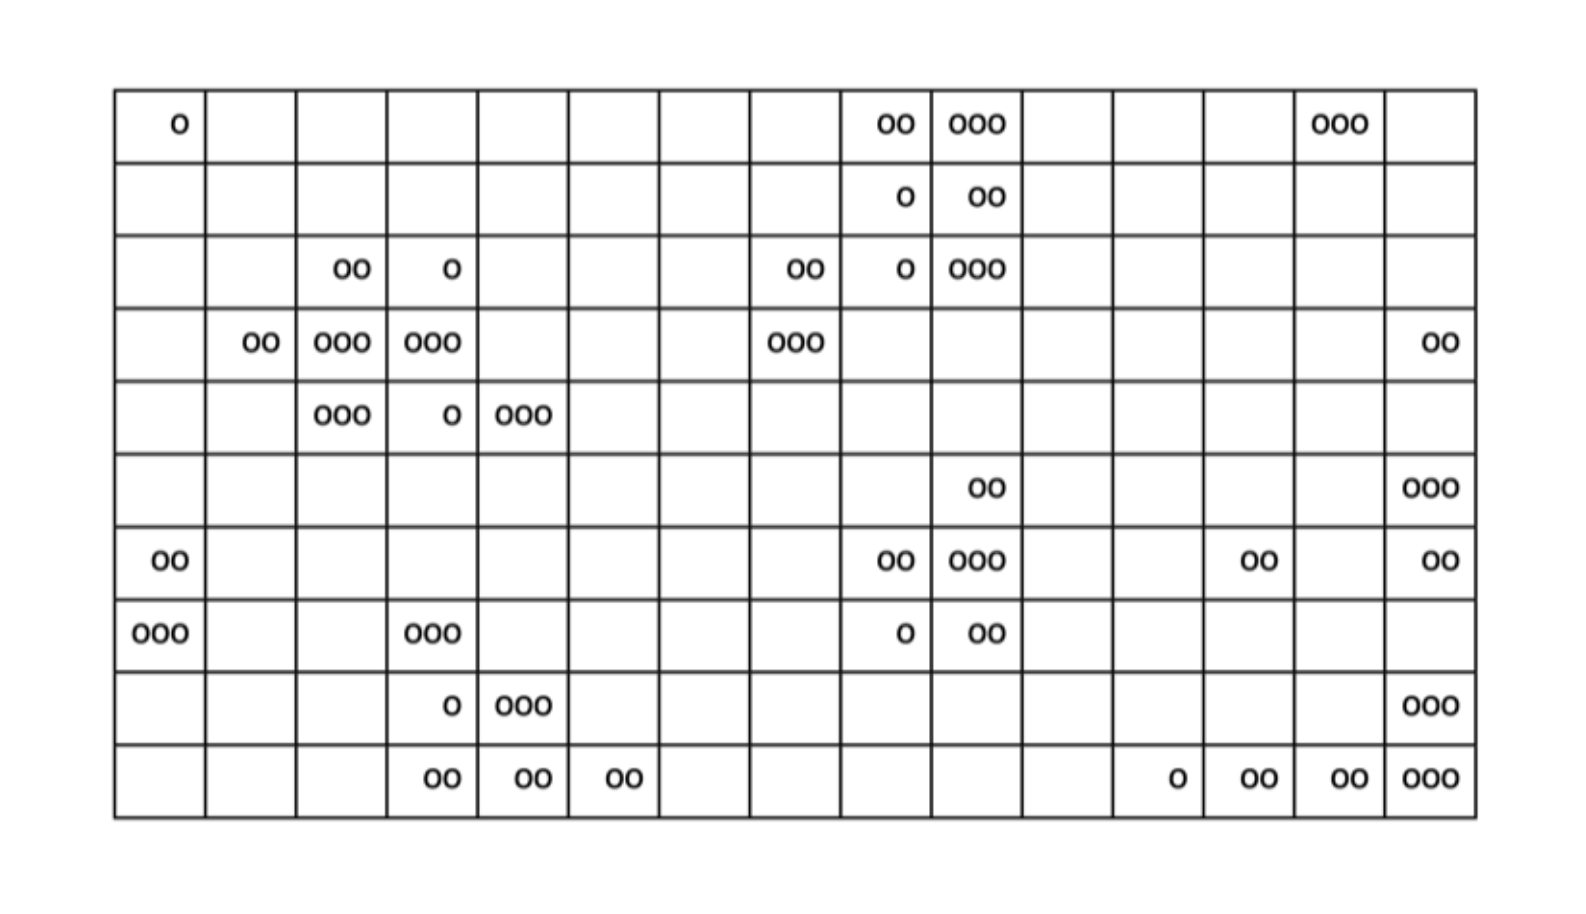
\includegraphics[width = .9\textwidth]{adaptivesampling.png}
    \end{center}
  \end{figure}
  
  \begin{enumerate}
    \item[a.] Select a simple random sample of size $n=8$ quadrats **with replacement**. 
    (NOT THAT YOU'LL DO THIS IN REAL LIFE, but if you only get empty clusters, you can draw 
    the sample again. In normal situations, you'd either give up or else get a larger sample size.\\
    \solution 
    We can use r to perform a simple random sample with replacement using the coordinates of each quadrat. \\
    \textbf{Code:}
\begin{center}
   \lstinputlisting{r3.txt}
\end{center}
\vspace{1in}

\item[b.]  For each unit in your sample, color in the resulting cluster if the rule is:
 Examine all squares to the N, S, E, W, NE, NW, SE, SW. Add any occupied quadrats to the cluster.
  Now repeat, searching around the newly added quadrats.  Don't add any empty quadrats.
    Stop when your cluster is surrounded by empty quadrats (or the boundary).\\
    \solution The following are the results of the adaptive sample from the SRS taken in the previous part, 
    \begin{figure}[H]
      \begin{center}
      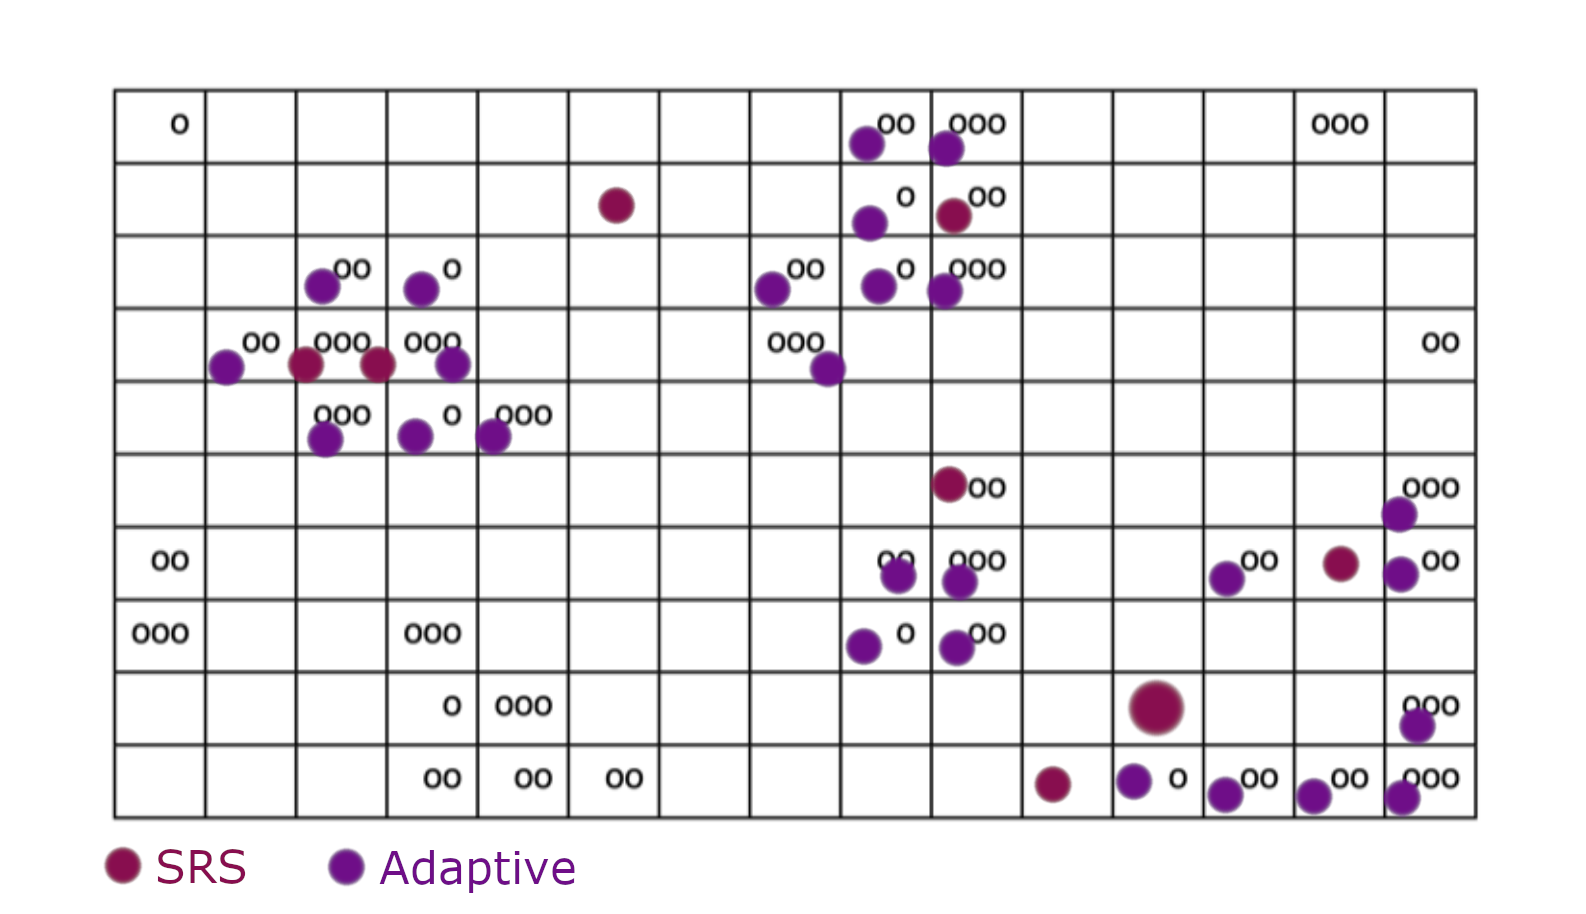
\includegraphics[width = .9\textwidth]{adaptivesampling01.png}
      \end{center}
    \end{figure}


    \item[c.]Write down the count for each cluster you hit, and the probability
     of getting that cluster in your sample. This is a type of probability
      proportional to size sampling.   NOTE:  If you get the same cluster
       more than once, you put it in your data as many times as you 'hit' the cluster.\\
       \solution The following is a .csv file containing coordinate information, flower count, and 
       probability for each of the sampled clusters under the adaptive sampling scheme. 
       \textbf{Code:}
       \begin{center}
          \lstinputlisting[basicstyle=\linespread{1}\ttfamily\small,columns=fullflexible]{AdaptiveSampling.csv}
       \end{center}
       \vspace{1in}

       \item[d.] Get an estimator for the total number of plants in the region and compute a 95 percent confidence interval for the total number of plants.  Is the estimator of the total unbiased?\\
       \solution Note that each unit sampled yields an unbiased estimator of $\tau$ with $\hat{\tau} = x_i/ P_i$ and similarly we can compute the variance. 
       Doing so in r, we get the following, \\
       \textbf{Code:}
       \begin{center}
          \lstinputlisting{r4.txt}
       \end{center}
       \vspace{1in}





  \end{enumerate}



  
\end{exercise}









\end{document}




















